%!TEX TS-program = xelatex

\documentclass {article}

\usepackage{xetexko}
\usepackage[a4paper]{geometry}
\usepackage[usenames,dvipsnames]{xcolor}
\usepackage{mathtools}
\usepackage{amsmath}
\usepackage{fontspec}
\usepackage{hyperref}
\usepackage{graphicx}
\usepackage{listings}
\usepackage{makeidx}
\usepackage{indentfirst}
\usepackage{tikz}
\usetikzlibrary{arrows,automata}


%\setmainfont {NanumMyeongjo}
\setmainfont {UnBatang}
\setmonofont[Scale=0.8]{DejaVu Sans Mono}

\lstdefinestyle{diff}{
  belowcaptionskip=1\baselineskip,
  breaklines=true,
  frame=L,
  xleftmargin=\parindent,
  showstringspaces=false,
  % Diffstart
  morecomment=[f][\color{gray}]{@@},
  % Diffincl
  morecomment=[f][\color{Green}]{+},
  % Diffrem
  morecomment=[f][\color{Red}]{-},
  basicstyle=\footnotesize\ttfamily,
}

\lstdefinestyle{customtxt}{
  belowcaptionskip=1\baselineskip,
  breaklines=true,
  frame=L,
  xleftmargin=\parindent,
  showstringspaces=false,
  basicstyle=\footnotesize\ttfamily,
}

\lstdefinestyle{customc}{
  belowcaptionskip=1\baselineskip,
  breaklines=true,
  frame=L,
  xleftmargin=\parindent,
  language=C,
  showstringspaces=false,
  basicstyle=\footnotesize\ttfamily,
  keywordstyle=\bfseries\color{green!40!black},
  commentstyle=\itshape\color{purple!40!black},
  identifierstyle=\color{blue},
  stringstyle=\color{orange},
}

\lstdefinestyle{customrs}{
  belowcaptionskip=1\baselineskip,
  breaklines=true,
  frame=L,
  xleftmargin=\parindent,
  showstringspaces=false,
  morekeywords={fn,let,mut,pub,use,impl,struct,unsafe,if,for},
  morecomment=[l]{//},
  morecomment=[n]{/*}{*/},
  basicstyle=\footnotesize\ttfamily,
  keywordstyle=\bfseries\color{green!40!black},
  commentstyle=\itshape\color{purple!40!black},
  identifierstyle=\color{blue},
  stringstyle=\color{orange},
}


\begin {document}

\title {Syscall 과 LSM Hook 을 이용해서 특정 프로세스 Kill 방지}
\input {../../reportauthor.tex}
\maketitle

\section {목적}
리눅스 커널의 task\_struct 에 tag 를 추가하여 프로세스에 tag 를 달고, 이를 LSM Hook 에서 읽어 프로세스 Kill 정책을 정함으로서

\vspace{\baselineskip}
\begin {itemize}
  \item 리눅스 커널 - 유저 간 데이터 교환 방법을 이해한다.
  \item 리눅스 커널 후킹을 이해한다.
  \item 리눅스 커널의 MAC과 이를 구현하기 위한 방법인 LSM을 이해한다.
\end {itemize}
\vspace{\baselineskip}

와 같은 목표를 달성한다.

\section {copy\_from\_user, copy\_to\_user}
시스템 콜은 유저로부터 메모리 주소를 받아오게 된다. 이 메모리 주소는 커널 영역에서 바로 쓰기엔 위험이 따른다. 해당 메모리 주소를 바로 사용할 경우, 유저는 시스템 콜을 이용해 커널 메모리 주소를 가르킴으로서, 커널 메모리에 액세스할 수 있는 취약점이 생기게 된다. 이를 방지하기 위해 리눅스 커널은 copy\_from\_user, copy\_to\_user 와 같은 유저 영역에서 커널 영역으로 (혹은 그 반대로) 데이터를 복사할 수 있는 함수를 지원한다. 이 함수가 호출되면, 내부적으로 access\_ok() 를 호출하여 이 주소가 액세스 가능하고, 유저 영역인지를 체크한 뒤, 데이터를 복사한다. 이 과정을 통해 유저가 시스템 콜에 악의적 데이터를 넣었을 때 커널 메모리를 보호하여 유저가 권한 상승하거나, 커널 패닉을 일으키는 것을 막을 수 있다.

또한 유저 어플리케이션은 커널 메모리에 바로 접근하지 못한다. 이는, 커널이 단순히 유저에게 커널 영역의 포인터를 넘겨준다고 해서 유저가 시스템 콜의 결과를 받아올 수 없다. 이를 해결하기 위해선 copy\_to\_user 를 통해 유저 영역으로 커널 영역의 데이터를 복사해 주어야 한다.

\section {시스템 콜 후킹}
\subsection {정적 후킹}
정적 후킹은 커널에 훅을 내장해서 후킹하려는 함수에 대한 동적인 수정 없이 함수가 훅을 호출하도록 하는 형태이다. 이의 대표적 예로 LSM 이 있다. LSM 의 훅은 리눅스 커널의 시스템 콜에 LSM 프레임워크를 호출하는 훅을 소스 단계에서 삽입함으로서 이루어진다. 시스템 콜이 LSM 프레임워크를 호출하게 되면, LSM은 보안 모듈이 로드되어 있을 때, 해당 호출을 보안 모듈의 권한 승인/거부 단으로 넘겨주어, 승인 여부를 받아 시스템 콜 동작을 계속할지, 실패시킬지를 결정시키는 형태로 작성되어 있다.

\subsection {동적 후킹}
동적 후킹은 커널에 훅을 내장하지 않고, 커널을 핫 패치해서 훅 코드를 끼워넣는 형태이다. 리눅스 커널의 KProbe 가 이를 이용해서 구현되어 있으며, KProbe 는 함수의 프롤로그를 패칭해서, 함수가 자신을 부르도록 패칭해 넣는다. 이를 통해 사전에 후킹 대상 함수에 미리 후킹 루틴을 작성하지 않아도, 동적으로 훅을 설치하고, 제거할 수 있다.
이 이외에도 리눅스의 시스템 콜만을 목표로 한다면 syscall\_table 에 저장된 함수 포인터를 공격하고자 하는 함수 포인터로 교체해서, 원래 시스템 콜 대신 후킹 루틴을 부르게 할 수도 있다.

\section {Mandatory Access Control}
LSM 의 훅은 리눅스 커널의 DAC - Discretionary Access Control 모델을 보완하기 위한 MAC 을 구현하는데 초점이 맞추어져 있다. DAC 에서는 사용자의 파일에 대한 소유권을 가지고 액세스를 제어하는데 반해, MAC 에서는 사용자 뿐만이 아니라 가동중인 프로세스와 같은 세부 사항까지 포함해서 파일 (객체) 에 대한 엑세스를 부분적으로 허용함으로서 더 세밀한 권한 설정을 가능하게 한다.

\section {LSM}
Linux Security Module 은 리눅스 커널에 MAC 을 구현하는 데 초점을 맞춘 프레임워크이다. 이는 상당수의 시스템 콜에 대해 정적 후킹을 지원하며, 프레임워크에 ``훅''을 등록함으로서 해당 시스템 콜로부터 MAC을 구현하는데 필요한 데이터들을 넘겨받고 이를 기반으로 하여 접근 승인 여부를 리턴하는 구조로 되어 있다.

\section {구현}
이 과제에서는 task\_struct 에 tag 변수를 달고, LSM hook selinux\_task\_kill() 에서 tag 를 확인, tag 가 특정 문자열로 시작 (이 과제에서는 NOTKILL)할 경우, kill system call 요청을 거부하도록 구현하였다. 추가적으로 과제의 요구사항 중에, printk 를 주석처럼 사용해서, 디버그 메시지를 출력하도록 하였으므로, 소스 코드의 주석은 printk() 내용으로 대체하였다.

아래는 이의 결과이다.
\lstinputlisting [style=customtxt]{dmesg.log}

\begin {figure}[h]
  \centering
  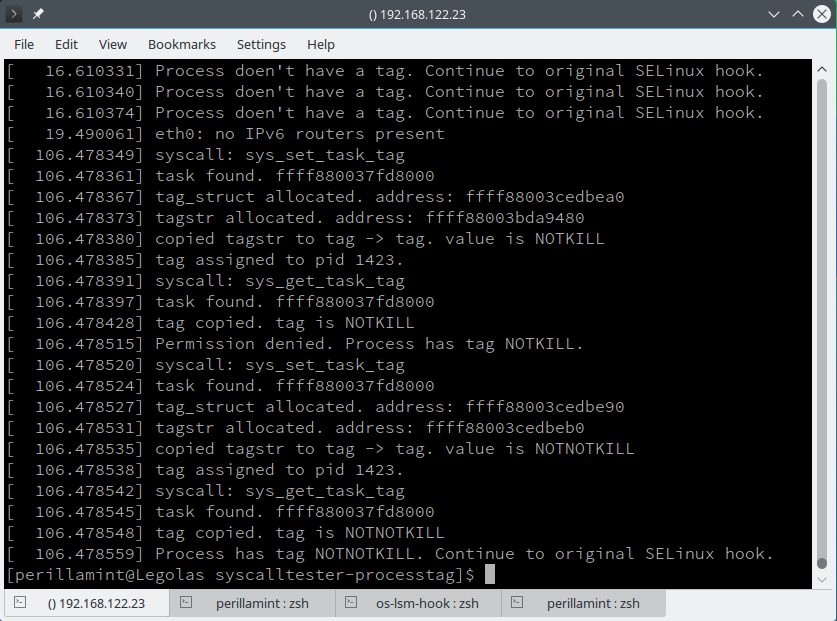
\includegraphics [width=120mm]{dmesg.png}
  \caption {킬 시도할 경우의 dmesg}
  \label{fig:dmesg}
\end {figure}

\section {발생한 문제점}
이번 과제는 유저 랜드에서 메모리 포인터를 커널 월드로 넘기는 작업이 포함되었다. 또한 이 넘어와야 할 데이터가 Null-terminated string 이므로, 이를 제대로 처리하지 않으면 Null-terminated string 을 가정하는 함수들에서 세그멘테이션 폴트가 일어날 가능성이 있으므로, 이를 체크하고 유저 랜드에서 복사해 온 데이터가 NULL을 포함하지 않으면 -EINVAL 을 리턴하도록 작성하였다. 

\section {부록 A - 소스 코드}
테스트 환경\newline
Guest OS:\newline
Kernel: Linux 2.6.35.6 AMD64\newline
Distro: Fedora 14\newline
\vspace{\baselineskip}
Host OS:\newline
Kernel: Linux 3.19.0-rc5\newline
Distro: Gentoo linux unstable AMD64\newline
Hypervisor: QEMU version 2.2.1 with KVM.\newline
\vspace{\baselineskip}
Host hardware:\newline
CPU: Intel i7-2670QM\newline

시스템 콜 테스트에 사용한 유저 앱.
\lstinputlisting [style=customc]{userapp.c}

패치 파일
\lstinputlisting [style=diff]{os-lsm-hook.patch}


\end {document}
